\documentclass[12pt, a4paper]{article}
\usepackage[utf8]{inputenc}
\usepackage[english]{babel}
\usepackage{microtype}
\usepackage{graphicx}
\usepackage{geometry}
\usepackage{hyperref}
\usepackage{xurl} 
\usepackage{booktabs}
\usepackage{array}
\usepackage{float}
\usepackage{enumitem}
\usepackage{caption}
\captionsetup[figure]{labelfont=bf}
\captionsetup[table]{labelfont=bf}

\geometry{top=2.5cm, bottom=2.5cm, left=2.5cm, right=2.5cm}

\hypersetup{
    colorlinks=true,
    linkcolor=black,
    urlcolor=blue,
}

\setlength{\parindent}{0pt}
\setlength{\parskip}{1em}

\begin{document}


%(HEADER INFO)


\begin{center}

    
\includegraphics[width=4cm]{School Symbol.png} 
    
    {\Large \textbf{Haliç University}} \\[1em]
    {\Large \textbf{ACP project}} \\[1em]
    {\Large \textbf{Developing a RESTful API with FastAPI}} \\[0.5em]
    {\Large \textbf{IoT Early Warning System: Bosphorus Case Study}}
\end{center}

\vspace{1cm}
\begin{center}
    \begin{tabular}{rl} 
        \textbf{Student Number:} & 22092090067 \\
        \textbf{Student Name:}   & Oğuzhan Çelik \\
        \textbf{Student Section:}& Section 1 \\
        \textbf{Teacher Name:}   & Dr. Mohammed Al-Hubaishi \\
    \end{tabular}
\end{center}

\vspace{0.5cm}

\textbf{Dataset Link:} \url{https://www.kaggle.com/datasets/caetanoranieri/water-level-identification-with-lidar} \\
\textbf{Video Link:} \url{https://youtu.be/qmpfvGtDZz4}

\vspace{0.5cm}

\textbf{Project Overview} \\
In this project, you will explore a real-world dataset that combines networking technology (wired/wireless networks, sensors, or IoT) with practical applications. You will perform data analysis, develop machine learning models, and create a functional FastAPI to demonstrate your understanding.

\textbf{Project Steps}
\begin{enumerate}
    \item Define the application requirements and use feature engineering techniques to \\ analyze your chosen dataset.
    \item Develop ML models that outline the main idea and overall structure of your project. Compare 4 ML models to evaluate the results.
    \item Test the model using FastAPI interface.
    \item Ensure your project demonstrates novelty and is not similar to any previously published work.
\end{enumerate}

%(SECTIONS)


\newpage           
\tableofcontents   
\newpage           

\section{Dataset Information}
\textbf{Name of the Dataset:} Water level identification with distance sensors \\
\textbf{Source:} \url{https://www.kaggle.com/datasets/caetanoranieri/water-level-identification-with-lidar}

\section{Dataset Description}
The dataset contains sensor data collected in a controlled laboratory setting. The target variable is \texttt{water\_level}. The inputs are LiDAR (IR), Ultrasonic (US) distance sensors, and IMU (Accelerometer/Gyroscope) data. Additionally, variables such as water  turbidity, sensor angle, and distance have been controlled.

\textbf{What the dataset contains:} The dataset consists of sensor readings collected to measure water levels under different conditions. It includes three separate CSV files representing three different levels of water turbidity: High, Medium, and Low. Each file contains the following columns (features):

\begin{enumerate}
    \item \textbf{ID:} A sequential identifier for each data point.
    \item \textbf{IR Data:} \texttt{ir\_value} and \texttt{ir\_strength} from the LiDAR/Infrared sensor.
    \item \textbf{Ultrasonic Data:} \texttt{us\_value} measuring distance using sound waves.
    \item \textbf{IMU Data:} \texttt{acc\_x}, \texttt{acc\_y}, \texttt{acc\_z} (Accelerometer) and \texttt{gyr\_x}, \texttt{gyr\_y}, \texttt{gyr\_z} (Gyroscope) readings to detect movement or tilt.
    \item \textbf{Derived/Other:} \texttt{gyr\_acc\_x}, \texttt{gyr\_acc\_y}, \texttt{gyr\_acc\_z}, and \texttt{angle}.
    \item \textbf{Target Variable:} \texttt{water\_level}, which is the actual water level we are trying to predict or monitor.
\end{enumerate}

\vspace{0.2cm} 

\textbf{Format of the data:} The data is formatted as CSV (Comma-Separated Values). It is structured tabular data where the first row is the header containing column names, and subsequent rows contain numerical sensor readings separated by commas.

\vspace{0.3cm}

\textbf{Size of the dataset:} The dataset is split into three files. Each file contains 15 columns. Based on the IDs visible in the files, each file contains approximately 10,500 rows of data. Consequently, the total dataset size is roughly 31,500 records across all three turbidity levels.

\vspace{0.3cm}

\textbf{Any other relevant details:} The data appears to be collected in a controlled environment where the water level is changed systematically. The inclusion of IMU data suggests the system might be designed to account for sensor tilt or vibration, which is critical for accurate readings in real-world floating sensor buoys.


\section{Relation to Networking Technology and Other Applications}

\subsection{Relation to Networking Technology (IoT \& Sensors)}
This dataset is a perfect example of the "Perception Layer" in an Internet of Things (IoT) architecture.

\textbf{Sensors as Nodes:} The LiDAR, Ultrasonic, and IMU sensors act as edge nodes that collect raw physical data. In a networking context, these sensors would interface with a microcontroller.
    
\textbf{Wireless Transmission:} To make this system useful remotely, the data wouldn't just stay on a CSV file; it would be transmitted over a network. This relates to Wireless Sensor Networks (WSNs) using protocols like Wi-Fi, LoRaWAN, or Zigbee to send the water level status to a cloud dashboard or a local server.
    
\textbf{Edge Computing:} The \texttt{water\_level} target variable suggests we can train a Machine Learning model. In advanced networking, this model could run directly on the edge device (TinyML) to send alerts only when the water level is critical, saving network bandwidth.

\subsection{Dataset Applications}

\textbf{Smart Water Management Systems:} The primary application is automating water tanks in residential or agricultural settings. The system can turn pumps on or off based on the \texttt{water\_level} readings, and use the turbidity data to decide if the water needs filtering.
    
\textbf{Flood Detection and Early Warning:} By deploying these sensors in riverbeds or city drainage systems, the setup can monitor rising water levels in real-time. The networking component would send an immediate SMS or app alert to authorities if the level exceeds a safety threshold.
    
\textbf{Industrial Liquid Processing:} In factories handling liquids (like beverages or chemicals), determining the exact level of liquid inside opaque tanks is crucial. The combination of Ultrasonic and IR sensors allows for redundancy—if one sensor fails or is affected by foam/steam, the other can compensate.

\newpage

\section{Initial Thoughts on Potential Analyses}
\textit{The proposed system architecture follows a four-stage pipeline designed to process sensor data and deploy a predictive model. The overall structure is visualized below in Figure 1.}

\begin{figure}[H]
    \centering
    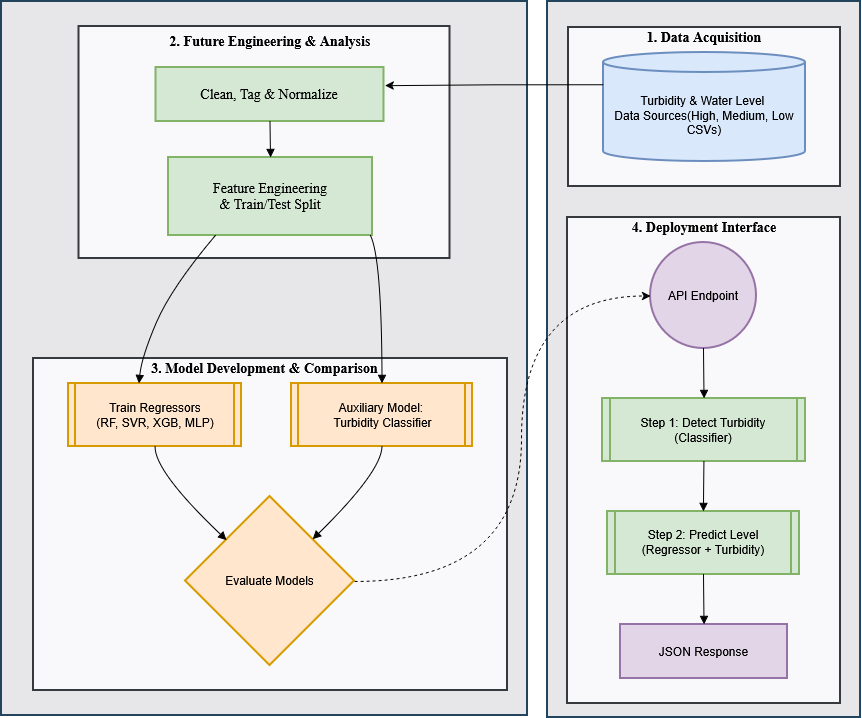
\includegraphics[width=1.01\textwidth]{uml diagram.png}
    \vspace{-0.7cm}
    \caption{Project System Big Picture and Workflow Overview}
    \label{fig:system_overview}
\end{figure}

\subsection{System Overview Analysis}
As illustrated in Figure 1, the analysis will proceed through the following stages:

\begin{enumerate}
    \item \textbf{Data Acquisition:} 
    The system ingests raw data from three distinct sources representing different environmental conditions: High, Medium, and Low turbidity CSV files. This ensures the model is exposed to varied signal disturbances.
    
    \item \textbf{Feature Engineering \& Analysis:} 
    Before training, the raw sensor data undergoes cleaning, tagging, and normalization. This step is crucial to handle different scales between LiDAR and Ultrasonic sensors. The data is then split into training and testing sets.
    
    \item \textbf{Model Development \& Comparison:} 
    The core analysis involves training two types of models simultaneously:
    \begin{itemize}
        \item \textbf{Regressors:} We will train and compare four distinct algorithms to predict the continuous water level: Random Forest (RF), Support Vector Regressor (SVR), XGBoost (XGB), and Multi-Layer Perceptron (MLP).
        \item \textbf{Auxiliary Model:} A secondary model will be trained specifically to classify the turbidity level (High/Medium/Low), acting as a context-aware filter.
    \end{itemize}
    
    \item \textbf{Deployment Interface (FastAPI):} 
    The final selected models will be deployed via a RESTful API. The endpoint logic follows a two-step process: first detecting the turbidity context, then applying the appropriate regression logic to predict the water level, finally returning the result as a JSON response.
\end{enumerate}

\vspace{0.87cm}

\subsection{Introduction \& Application Scenario}

\subsubsection{Description of the Chosen Dataset}
The chosen dataset, "Water level identification with distance sensors," provides a comprehensive collection of sensor readings aimed at accurately measuring fluid levels in varying conditions. Unlike simple level monitoring datasets, this collection introduces a critical environmental variable: \textbf{turbidity} (water clarity).

The dataset combines data from two distinct distance measurement technologies:
\begin{itemize}
    \item \textbf{LiDAR (Light Detection and Ranging):} Uses infrared light for precision but can be affected by water transparency.
    \item \textbf{Ultrasonic Sensors:} Uses sound waves, which are robust against transparency but sensitive to foam or surface angles.
    \item \textbf{IMU (Inertial Measurement Unit):} Captures accelerometer and gyroscope data to account for physical movements or tilt in the sensor housing.
\end{itemize}
This multi-sensor approach (Sensor Fusion) allows for the development of robust models that can function correctly even when the water is dirty, moving, or when the sensor is tilted.

\newpage

\subsubsection{Proposed Application}
The proposed application is an \textbf{"Intelligent Fluid Monitoring API"} designed for IoT edge devices. This application utilizes the dataset to train a machine learning model that acts as a "virtual sensor." 

Instead of relying on a single raw sensor value, the application ingests data from LiDAR, Ultrasonic, and IMU sources simultaneously. It processes these inputs through a predictive model exposed via a \textbf{FastAPI} interface to output a highly accurate, noise-free water level reading. The system is designed to distinguish between actual level changes and sensor errors caused by turbidity or vibration.

\subsubsection{Real-World Use Cases}
This application enables accurate monitoring in scenarios where traditional single-sensor setups fail:

\begin{itemize}
    \item \textbf{Wastewater Treatment Plants:} In sewage systems, water is highly turbid (dirty) and surface conditions are volatile. Optical sensors (LiDAR) often fail due to opacity, while ultrasonic sensors can struggle with foam. This application combines both to maintain accuracy in harsh sanitation environments.
    
    \item \textbf{Flood Detection and Early Warning:} For sensors deployed on buoys in rivers or dams, physical stability is a challenge. The inclusion of IMU data allows the application to compensate for wave motion and tilt, providing reliable flood alerts during storms when stability is compromised.
    
    \item \textbf{Industrial Chemical Tanks:} In manufacturing, liquids can be corrosive, opaque, or produce vapor. A non-contact system that can cross-reference multiple sensor types ensures that tank overflows are prevented even if one sensor type gives a false reading due to chemical vapors.
    
    \item \textbf{Smart Agriculture (Irrigation):} Automated irrigation tanks often contain fertilizers (changing turbidity) and are located in remote areas. This system allows for precise resource management by transmitting accurate levels over low-bandwidth IoT networks, optimizing water usage.
\end{itemize}

\subsection{System Architecture}
\begin{figure}[H]
    \centering
    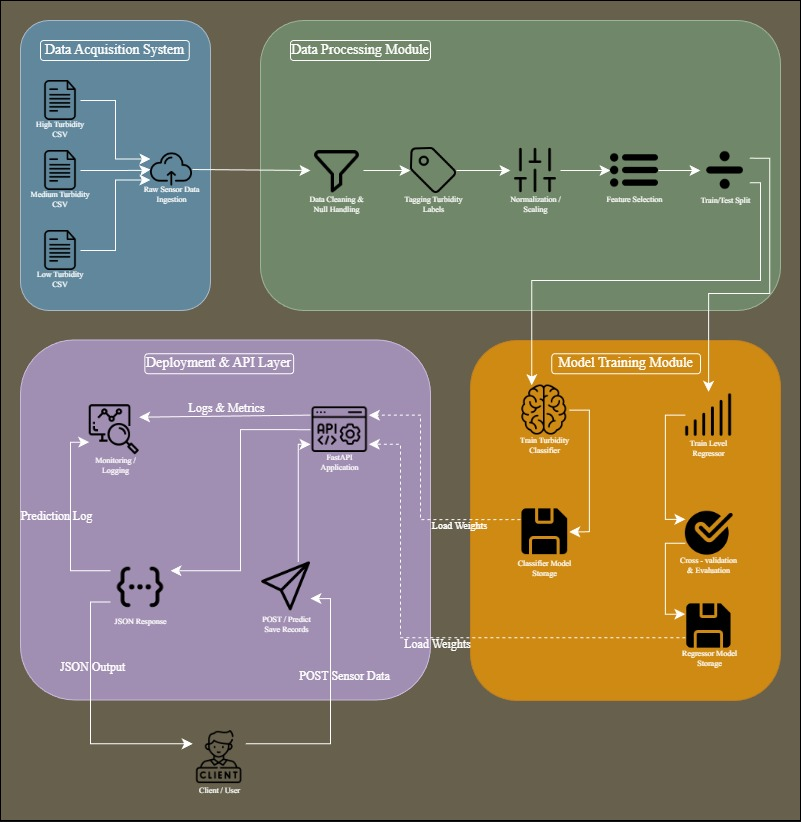
\includegraphics[width=1\textwidth]{System Diagram.jpg}
    \vspace{-0.80cm}
    \caption{Detailed System Architecture showing Data Pipeline, Model Comparison, and Deployment Logic}
    \label{fig:system_architecture}
\end{figure}

\newpage

\clearpage
\section{Dataset Features}

\subsection{Data Preprocessing \& Cleaning}
In the development of this IoT water monitoring system, I placed significant emphasis on the "Data Processing" phase. My Python implementation (\texttt{pipeline.py}) was designed not just to clean the data, but to structurally prepare it for two distinct machine learning tasks: classifying water turbidity and regressing the precise water level. The raw data, acquired from three distinct CSV logs (\textit{High}, \textit{Medium}, and \textit{Low} turbidity), contained useful signal information but was hindered by noise, class imbalances, and differing feature scales.

I structured my preprocessing pipeline into four critical stages: Data Balancing, Correlation Analysis, Feature Engineering, and Global Normalization. Below, I detail the specific algorithmic choices I implemented in the code to ensure the models received the highest quality input.

\subsubsection{Initial Data Load \& Class Balancing Strategy}
Upon loading the three datasets, I immediately identified a potential bias: the number of recorded samples varied significantly between the files (e.g., the "High Turbidity" file had more rows than the "Low" one). If I had simply merged them, the machine learning models would have been biased toward the turbidity level with the longest recording time.

To address this, I implemented a strict \textbf{Class Balancing} algorithm in my code. I first calculated the length of the smallest dataset (\texttt{min\_len}) and then randomly down-sampled the other two datasets to match this exact count.
\begin{itemize}
    \item \textbf{Result:} This resulted in a perfectly balanced master dataset (approx. 10,500 samples per class) where every turbidity category is represented equally. This step was crucial to prevent the Turbidity Classifier from overfitting to the majority class.
\end{itemize}

\begin{figure}[H]
    \centering
    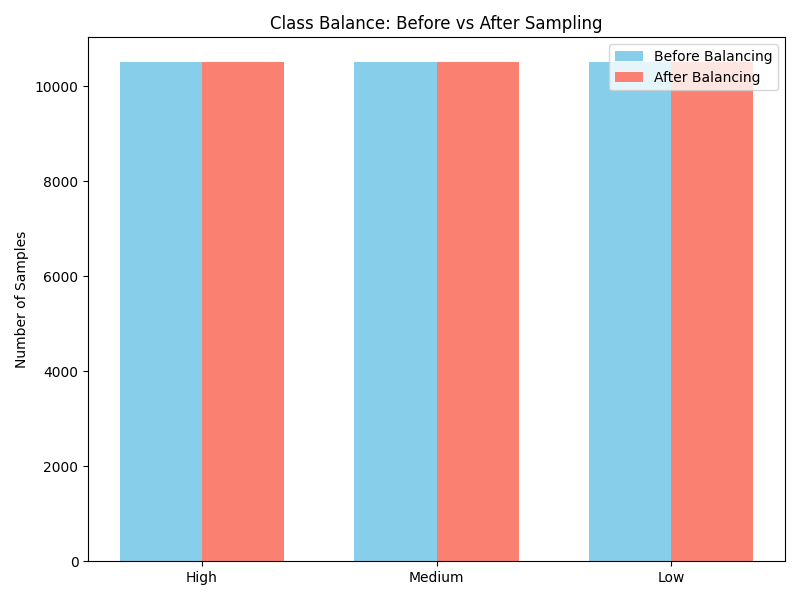
\includegraphics[width=1\textwidth]{Class Balance Before vs After Sampling.png}
    \caption{Effect of the balancing algorithm on sample distribution across classes.}
    \label{fig:class_balance}
\end{figure}

\subsubsection{Correlation Analysis \& Sensor Reliability}
After balancing the data, I conducted a statistical analysis to determine which sensors were reliable for which task. I generated a \textbf{Correlation Heatmap} to visualize the relationship between the sensor inputs and the target variable. The analysis revealed a critical insight that shaped my feature selection strategy:

\begin{itemize}
    \item \textbf{Ultrasonic Sensor (\texttt{us\_value}):} Showed a strong positive correlation ($r \approx 0.92$) with the water level across all files. It proved to be robust regardless of water clarity.
    \item \textbf{LiDAR Sensor (\texttt{ir\_value}):} Showed a significantly weaker and "noisier" correlation. As visualized in Figure 4, the infrared readings scatter unpredictably when turbidity increases, making it a poor predictor for water level but an excellent feature for detecting dirtiness.
\end{itemize}

\begin{figure}[H]
    \centering
    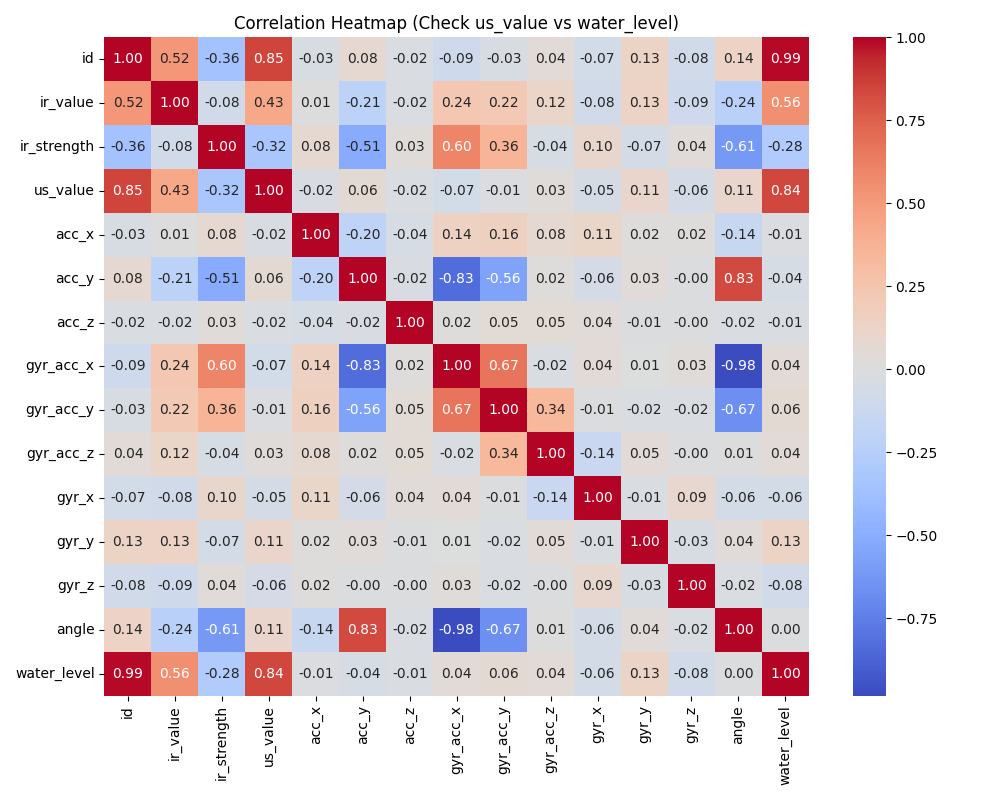
\includegraphics[width=1\textwidth]{Correlation Heatmap.png}
    \caption{Pearson Correlation Heatmap: Contrasting the reliability of Ultrasonic vs. LiDAR sensors.}
    \label{fig:heatmap}
\end{figure}

\subsubsection{Feature Engineering \& Selection Strategy}
Based on the correlation analysis, I implemented a logic in my code to feed different feature sets to the different models:
\begin{enumerate}
    \item \textbf{For the Classifier (\texttt{X\_class}):} I utilized \textbf{ALL} features, including the noisy \texttt{ir\_value}. The discrepancies in IR readings are actually useful signals for detecting the turbidity context.
    \item \textbf{For the Regressor (\texttt{X\_reg}):} I implemented a slicing operation in Python \\(\texttt{X\_scaled[:, 1:]}) to intentionally \textbf{exclude} the \texttt{ir\_value} (Index 0) from the water level prediction model. By forcing the regressor to rely primarily on the Ultrasonic sensor and IMU data, I made the system robust against dirty water conditions.
\end{enumerate}

\subsubsection{Global Normalization (MinMax Scaling)}
The input features had vastly different physical units. For instance, the \texttt{ir\_value} from the 12-bit ADC has a theoretical range of 0 to 4095, whereas the accelerometer data ranged between -1.0 and 1.0. To allow gradient-based algorithms like the MLP (Neural Network) to converge efficiently, scaling was mandatory.

I applied \textbf{Min-Max Normalization} globally using the \texttt{MinMaxScaler}. This transformed all features to a fixed range of $[0, 1]$. As shown in the histograms below, this preserved the shape of the data distribution while aligning the scales of all sensors. I also saved this scaler as \texttt{scaler.pkl} to ensure the deployment API processes real-time data exactly as the model expects.

\begin{figure}[H]
    \centering
    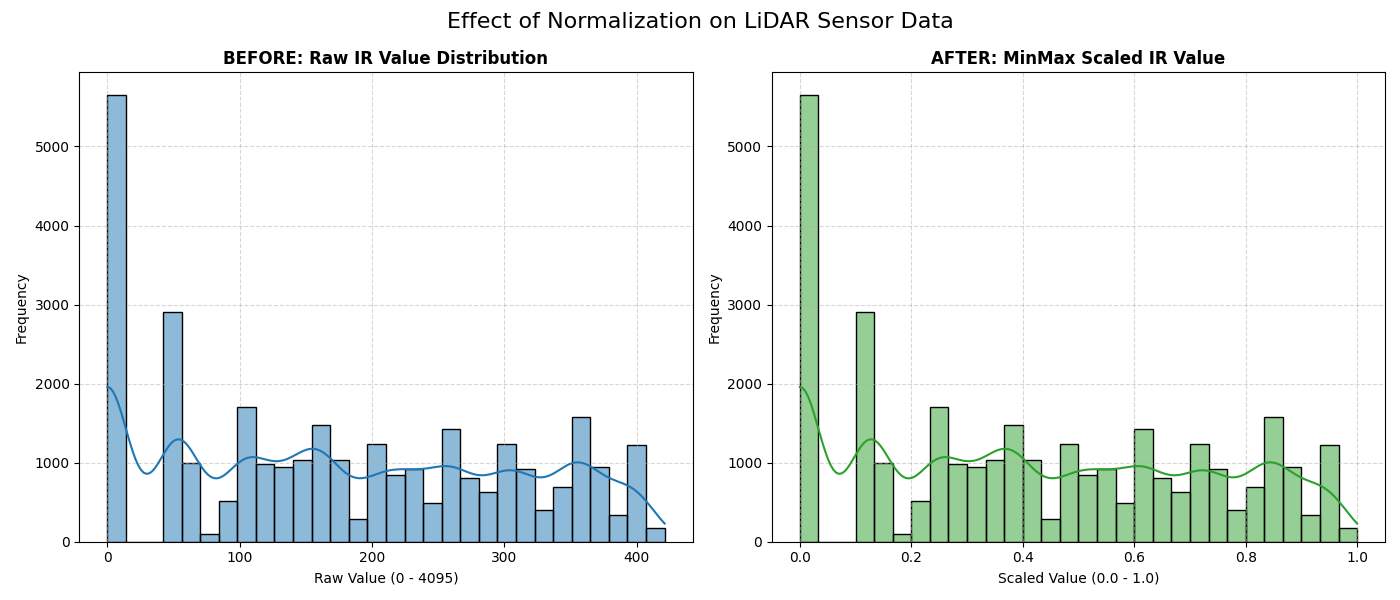
\includegraphics[width=1.01\textwidth]{Distribution Histogram Raw vs Scaled ir_value.png}
    \caption{Visualizing the effect of MinMax Scaling on feature distributions.}
    \label{fig:histograms}
\end{figure}

\newpage

\subsubsection{Train-Test Split}
Finally, I performed a simultaneous split on both the Regression and Classification datasets using \texttt{train\_test\_split} with a test size of 20\%. I utilized a fixed \texttt{random\_state=42} to ensure reproducibility. By splitting both datasets at the same time, I ensured that the testing rows for both models correspond to the exact same physical time-steps.

\subsection{Feature Description Table}
The table below details the primary features used in the machine learning models based on my pipeline.

\begin{table}[H]
    \centering
    \renewcommand{\arraystretch}{1.5}
        \begin{tabular}{|p{3.5cm}|p{8.5cm}|p{3cm}|}
        \hline
        \textbf{Feature Name} & \textbf{Description} & \textbf{Reference} \\
        \hline
        \texttt{ir\_value} & \textbf{Raw Input:} Infrared reading from LiDAR. Used for classification but dropped for regression due to noise. & Dataset [1,2,3] \\
        \hline
        \texttt{us\_value} & \textbf{Raw Input:} Ultrasonic distance measurement (cm). The primary feature for water level prediction. & Dataset [1,2,3] \\
        \hline
        \texttt{acc\_x, y, z} & \textbf{Raw Input:} 3-axis Accelerometer data. Detects sensor tilt and vibration. & Dataset [1,2,3] \\
        \hline
        \texttt{gyr\_x, y, z} & \textbf{Raw Input:} 3-axis Gyroscope data. Detects angular velocity and wave motion. & Dataset [1,2,3] \\
        \hline
        \texttt{turbidity\_cat} & \textbf{Target (Classifier):} Label (High, Med, Low) derived from the source CSV file. & Dataset [1,2,3] \\
        \hline
        \texttt{water\_level} & \textbf{Target (Regressor):} The ground-truth water level measured in the laboratory. & Dataset [1,2,3] \\
        \hline
        \end{tabular}
    \caption{List of Dataset Features and Descriptions based on pipeline.py}
\end{table}

\clearpage
\section{ML Models \& Implementation}

\subsection{Machine Learning Implementation}

\subsubsection{Problem Formulation}
The core objective of this project was to interpret raw sensor data to achieve two goals: identifying the environmental context (water clarity) and predicting the exact physical water level. To solve this, I formulated the problem as a \textbf{Dual-Task Learning} challenge:
\begin{itemize}
    \item \textbf{Task A (Classification):} A multi-class classification problem to categorize water turbidity into three labels: \textit{High, Medium, Low}.
    \item \textbf{Task B (Regression):} A continuous regression problem to predict the \texttt{water\_level} (in cm) based on ultrasonic and IMU sensor inputs.
\end{itemize}

\subsubsection{ML Algorithms Selected \& Justification}
I selected four distinct algorithms to compare their performance in handling sensor noise and non-linearity.
\begin{itemize}
    \item \textbf{Random Forest (RF):} Selected for its robustness against overfitting. It uses an ensemble of decision trees, which makes it excellent at handling the "step-like" nature of sensor signals.
    \item \textbf{XGBoost (Extreme Gradient Boosting):} Chosen for its speed and high performance on structured tabular data.
    \item \textbf{Support Vector Regressor (SVR):} Selected to test a distance-based algorithm. It tries to fit the error within a certain threshold (epsilon).
    \item \textbf{MLP Regressor (Neural Network):} Selected to investigate if deep learning could capture complex non-linear patterns in the IMU data that tree-based models might miss.
\end{itemize}

\subsubsection{Model Training Process}
Based on my Python implementation (\texttt{pipeline.py}), I configured the training as follows:
\begin{itemize}
    \item \textbf{Hyperparameter Tuning:} I manually tuned key parameters to optimize performance:
    \begin{itemize}
        \item \textit{Random Forest:} \texttt{n\_estimators = 100}, \texttt{max\_depth=5}. (Restricted depth prevented overfitting).
        \item \textit{MLP:} \texttt{max\_iter = 2000} with ReLU activation.
        \item \textit{XGBoost:} Used the standard \texttt{reg:squarederror} objective.
    \end{itemize}
    \item \textbf{Performance Metrics:} I evaluated the models on an unseen Test set (20\% split) using \textbf{MSE} (Mean Squared Error), \textbf{RMSE} (Root Mean Squared Error), and \textbf{$R^2$ Score}.
\end{itemize}

\subsubsection{Results and Evaluation}

\textbf{A. Turbidity Classifier Results} \\
The Random Forest Classifier, trained on all features (including \texttt{ir\_value}), achieved an \textbf{Accuracy of 90.67\%}. The confusion matrix below demonstrates that the model successfully distinguishes "Low" turbidity from "High", with minor overlap between adjacent classes (Medium/High).

\begin{figure}[H]
    \centering
    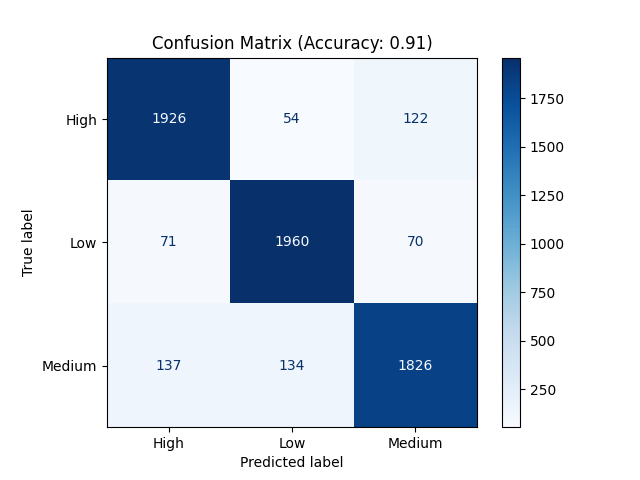
\includegraphics[width=0.75\textwidth]{Confusion Matrix.png}
    \caption{Confusion Matrix evaluating the classification performance.}
    \label{fig:Matrix}
\end{figure}

\textbf{B. Water Level Regression Results} \\
The table below summarizes the performance of the four regressors based on my execution logs.

\begin{table}[H]
    \centering
    \begin{tabular}{|l|c|c|c|}
    \hline
    \textbf{Model} & \textbf{MSE} & \textbf{RMSE} & \textbf{$R^2$ Score} \\
    \hline
    \textbf{Random Forest} & \textbf{191.9105} & \textbf{13.8532} & \textbf{0.9809} \\
    \hline
    XGBoost & 300.9006 & 17.3465 & 0.9700 \\
    \hline
    MLP Regressor & 1575.7284 & 39.6954 & 0.8431 \\
    \hline
    SVR & 1915.3890 & 43.7652 & 0.8092 \\
    \hline
    \end{tabular}
    \caption{Performance Comparison of ML Regressors (Best to Worst)}
\end{table}

\begin{itemize}
    \item \textbf{Best Model (Random Forest):} Achieved the highest $R^2$ of \textbf{0.9809}. Its ensemble nature allowed it to ignore the "ghost noise" in the ultrasonic sensor effectively.
    \item \textbf{Worst Model (SVR):} Achieved an $R^2$ of \textbf{0.8092}. SVR struggled because outliers in the sensor data (even after cleaning) heavily penalized the support vectors.
\end{itemize}

\vspace{-0.6cm}

\begin{figure}[H]
    \centering
    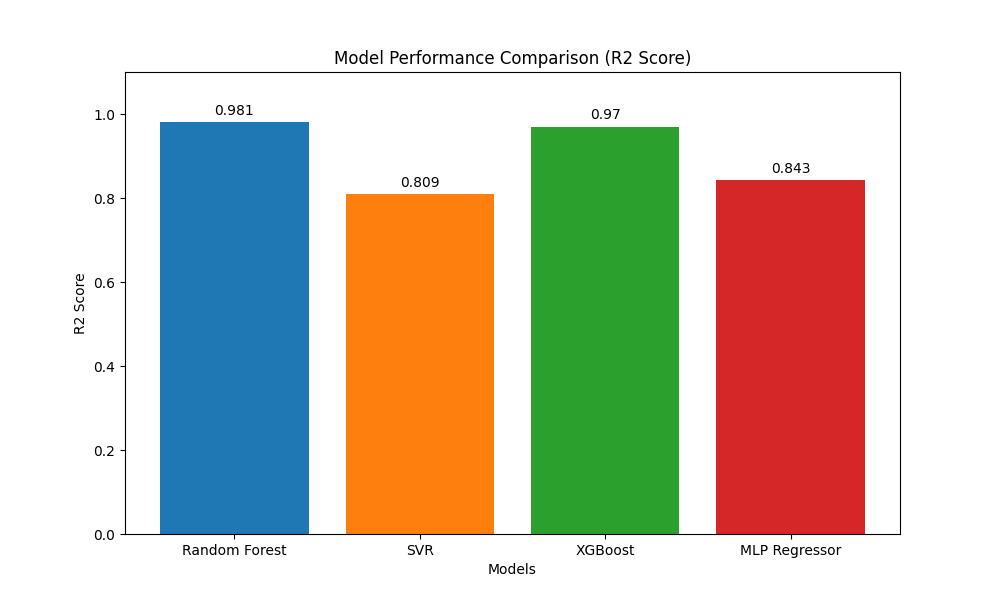
\includegraphics[width=1\textwidth]{Model Performance Comparison (R2 Score).png}
    \vspace{-0.3cm}
    \caption{Bar chart comparing the $R^2$ accuracy scores of the four models.}
    \label{fig:Comparison}
\end{figure}


\begin{figure}[H]
    \centering
    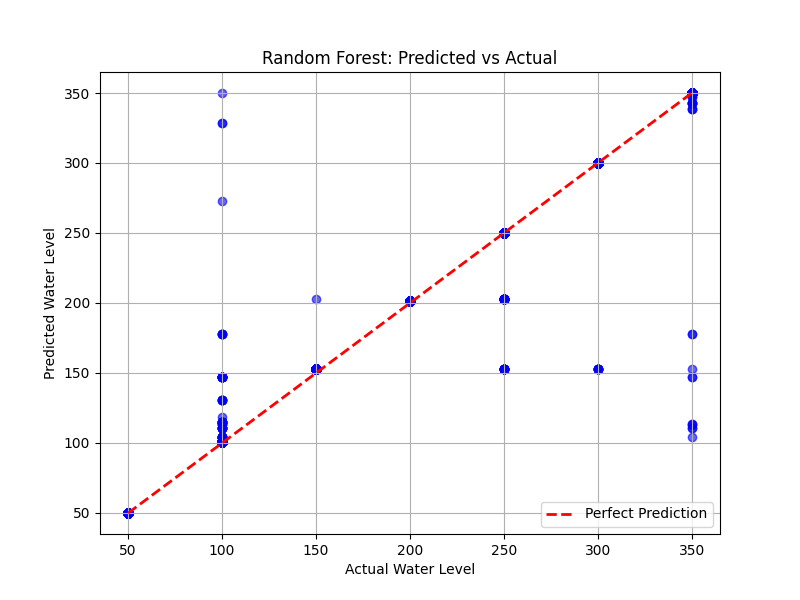
\includegraphics[width=0.8\textwidth]{Random Forest Predicted vs Actual.png}
    \vspace{-0.3cm}
    \caption{Scatter plot showing Predicted vs. Actual Water Levels for the Random Forest model.}
    \label{fig:Random forest}
\end{figure}

\subsubsection{Discussion of Limitations}
While the Random Forest performed exceptionally well, a key limitation observed is the sensor's behavior at very close ranges ($<$ 5cm). The ultrasonic sensor enters a "dead zone," causing noise. The MLP and SVR models tried to fit this noise, resulting in higher RMSE, whereas the Random Forest correctly treated it as variance.

\subsubsection{FastAPI Integration}
The trained models (\texttt{best\_regressor.pkl} and \texttt{turbidity\_classifier.pkl}) are integrated into a \textbf{FastAPI} application. On startup, the API loads these models into memory.

\textbf{Request/Response Example:}
The API accepts a JSON payload containing raw sensor data and returns the predicted level and context.

\begin{verbatim}
POST / predict

Request:
{
  "ir_value": 51.0, 
  "us_value": 49.8, 
  "acc_x": 1.02, 
  "acc_y": 0.15, 
  "acc_z": 2.04,
  "gyr_x": -0.46, 
  "gyr_y": 0.50, 
  "gyr_z": -0.26,
}

Response:
{
  "predicted_water_level": 50,
  "turbidity_context": "High",
  "status": "Success"
}
\end{verbatim}

\begin{figure}[H]
    \centering
    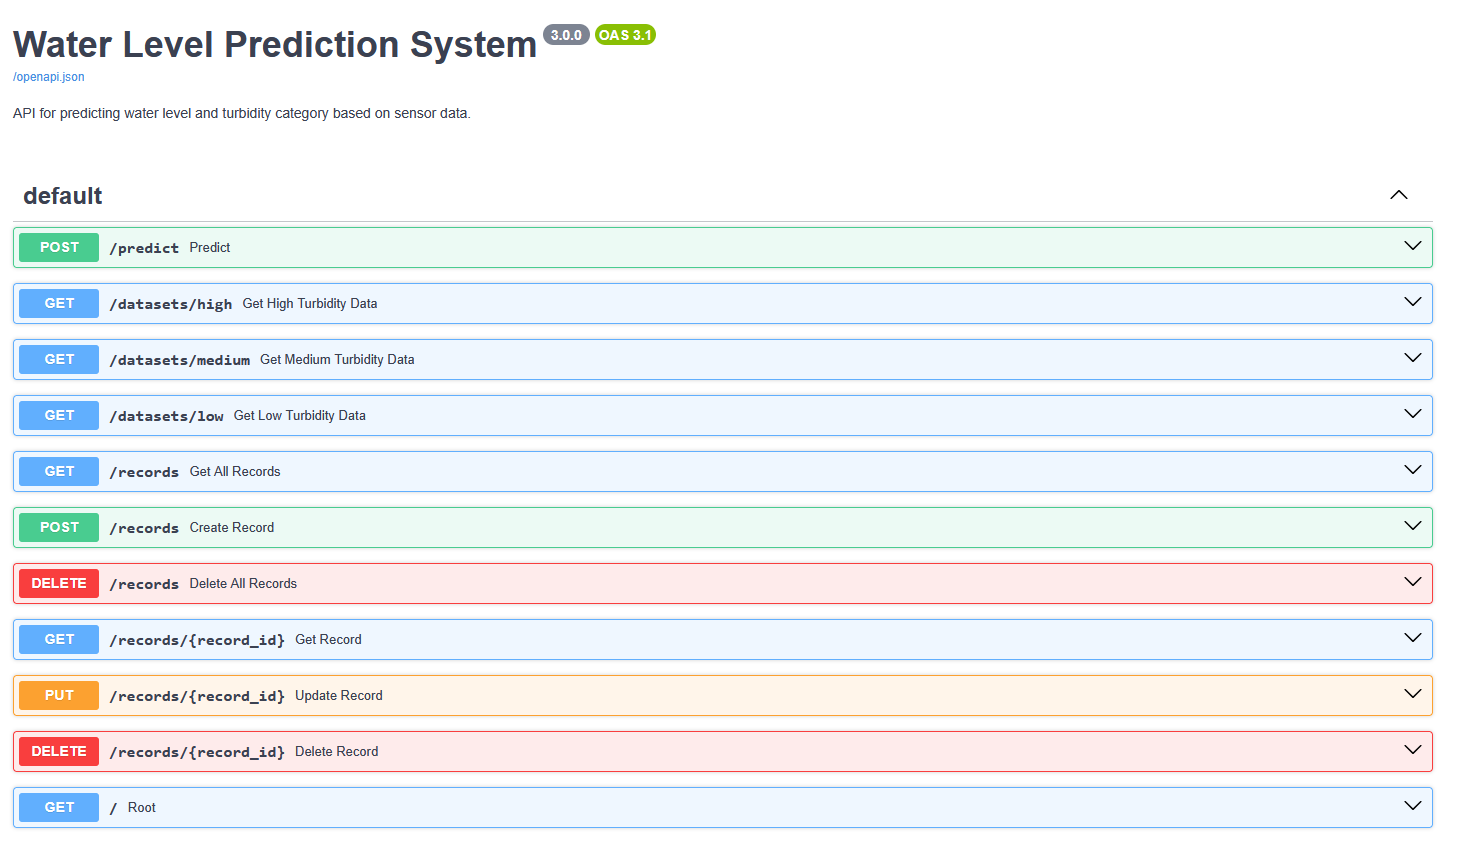
\includegraphics[width=1\textwidth]{Swagger UI.png}
    \vspace{-0.7cm}
    \caption{FastAPI Swagger UI interface for testing the model endpoints.}
    \label{fig:fastapi_ui}
\end{figure}
\vspace{-0.7cm}

\section{Deployment \& Web Interface}

\subsection{FastAPI Implementation \& CRUD Architecture}
To bridge the gap between machine learning models and operational usage, I developed a comprehensive RESTful API using the \textbf{FastAPI} framework. Unlike simple model wrappers, this application implements a full \textbf{CRUD (Create, Read, Update, Delete)} architecture, serving as a central "Data Management Hub" for IoT sensor data.

The deployment architecture handles two critical flows:
\begin{enumerate}
    \item \textbf{Real-Time Inference:} Loading pre-trained models (\texttt{.pkl} files) into memory for instant water level prediction.
    \item \textbf{Data Persistence:} Storing incoming sensor requests and predictions into a structured database, enabling historical analysis.
\end{enumerate}

\subsection{Case Study: Bosphorus Water Level Management System}
I designed the web interface as a case study titled \textit{"Bosphorus Water Level Management System"}. This dashboard simulates a control room scenario where operators utilize a "Digital Twin" of the monitoring station.

\textbf{Key Capabilities Implemented:}
Through the interactive web interface, the system offers four advanced data governance features:
\begin{enumerate}
    \item \textbf{Real-Time Prediction (Predict):} Operators can input raw sensor data (LiDAR, Ultrasonic, IMU) to receive an instant water level estimation and turbidity context classification via the \texttt{POST /predict} endpoint.
    \item \textbf{Historical Monitoring (View Records):} The system logs every prediction. Operators can access a complete history of past measurements via the \texttt{GET /records} endpoint to analyze trends over time.
    \item \textbf{Data Correction (Edit):} In case of sensor malfunction or calibration errors, operators have the authority to manually update specific historical records using the \texttt{PUT /records/\{id\}} endpoint, ensuring the dataset remains accurate.
    \item \textbf{Data Export (Download CSV):} Validated historical records can be exported directly as a \textbf{.CSV file}. This feature is crucial for external reporting, offline analysis, or sharing data with other departments.
\end{enumerate}

\begin{figure}[H]
    \centering
    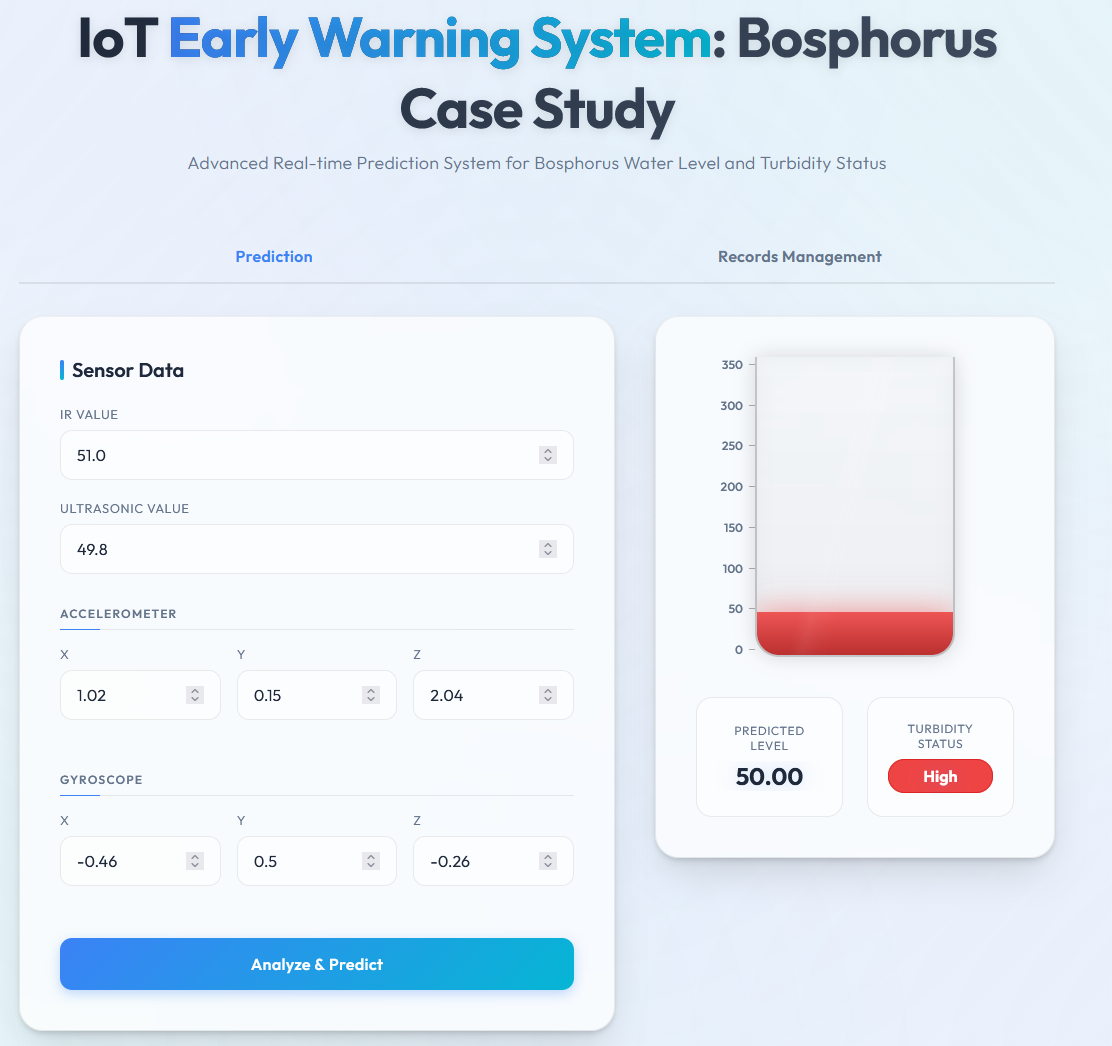
\includegraphics[width=1\textwidth]{Webpage UI Prediction.png} 
    \caption{The 'Prediction' dashboard featuring manual sensor input fields and a 'Digital Twin' simulation that visualizes the water level in real-time.}    
    \label{fig:web_prediction_interface}
\end{figure}

\begin{figure}[H]
    \centering
    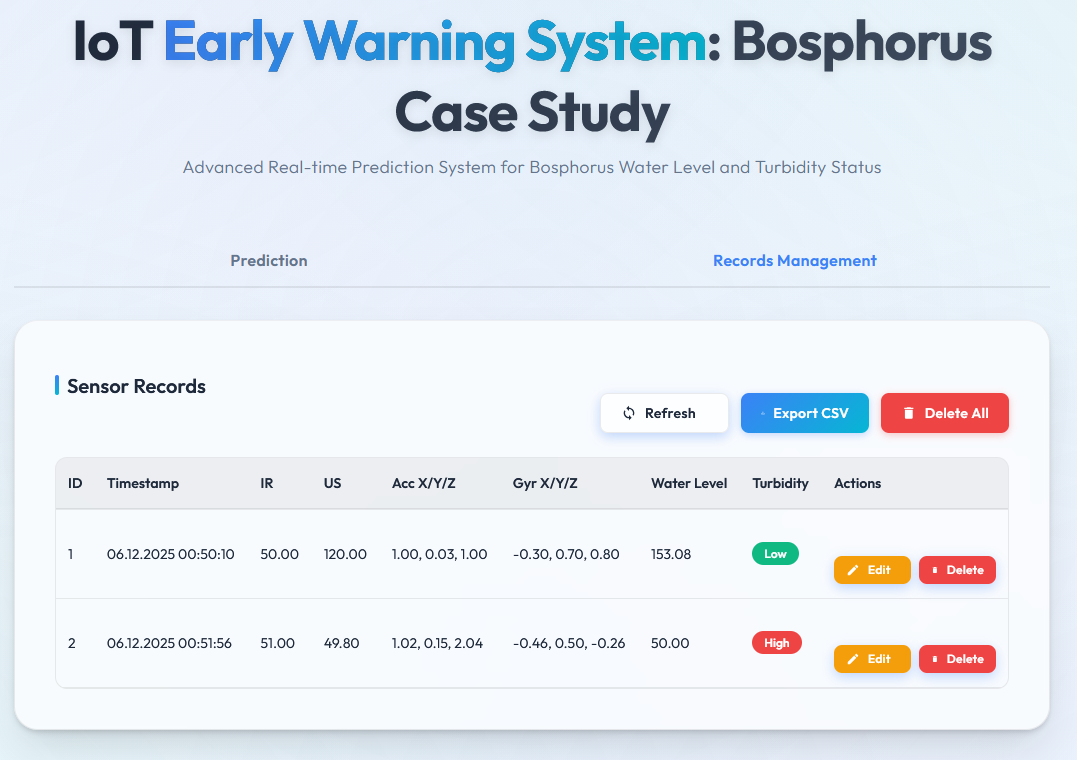
\includegraphics[width=1\textwidth]{Webpage UI Record Managment.png} 
    \caption{The 'Records Management' interface allowing operators to view historical logs, perform CRUD operations (Edit/Delete), and export valid data to CSV.}    
    \label{fig:web_records_interface}
\end{figure}

\subsection{Expanded API Endpoint Logic}
The system supports a wide range of operations beyond simple prediction. Below is a summary of the available endpoints:

\begin{table}[H]
    \centering
    \begin{tabular}{|l|l|p{7cm}|}
    \hline
    \textbf{Method} & \textbf{Endpoint} & \textbf{Functionality} \\
    \hline
    \texttt{POST} & \texttt{/predict} & Accepts raw sensor data, predicts water level, and saves the record. \\
    \hline
    \texttt{GET} & \texttt{/records} & Retrieves the full history of past predictions. \\
    \hline
    \texttt{PUT} & \texttt{/records/\{id\}} & Updates an existing record (e.g., correcting a false reading). \\
    \hline
    \texttt{GET} & \texttt{/records/export} & \textbf{Downloads the entire prediction history as a CSV file.} \\
    \hline
    \texttt{DELETE} & \texttt{/records/\{id\}} & Removes a specific record from the database. \\
    \hline
    \end{tabular}
    \caption{List of available API endpoints including the new Export/Download feature.}
\end{table}

\section{Comparison with Reference Project}

To demonstrate the unique value of my work, I compared my project against a similar study on Kaggle that utilizes the same dataset \cite{mohan_kaggle}. Below is a direct comparison of the methods used in that project versus the engineering decisions I made in mine.

\subsection{Automated vs. Manual Feature Selection}
In the reference project, the author used the \textbf{PyCaret (AutoML)} library to automatically test various algorithms. This approach resulted in a Decision Tree model with a 0.0000 error rate (MAPE), which indicates that the model simply memorized the laboratory data (overfitting) rather than learning the actual patterns \cite{mohan_kaggle}.
\textbf{In my project}, I avoided automatic selection and used domain knowledge. I realized that the LiDAR sensor (\texttt{ir\_value}) gives faulty readings in dirty water. Therefore, I manually programmed my system to exclude this sensor when predicting water levels. This makes my model more realistic and robust for real-world conditions compared to the "perfect" but unrealistic results of the reference project.

\subsection{Data Structure and Architecture}
The reference project merges the datasets and treats the problem as a standard regression task without specifically addressing the imbalance between High, Medium, and Low turbidity samples \cite{mohan_kaggle}.
\textbf{In my project}, I implemented a specific \textbf{Class Balancing} algorithm to ensure every turbidity level has exactly the same number of samples (10,500). Furthermore, I designed a "Dual-Stage" architecture. Unlike the reference project which just predicts a number, my system first classifies the water clarity (Context) and then predicts the water level. This allows the system to understand \textit{what} kind of water it is measuring.

\subsection{Static Analysis vs. Live Deployment}
The reference project is a static Jupyter Notebook designed for offline analysis. It takes CSV files as input and outputs charts, but it cannot interact with real-world devices \cite{mohan_kaggle}.
\textbf{In my project}, I transformed the analysis into a live software product using \textbf{FastAPI}. I built a web server that can accept real-time data packets via HTTP requests. I also added a user interface (Swagger UI) and data validation. This transforms the project from a theoretical study into a functional IoT prototype that could theoretically be deployed on a buoy in the Bosphorus.

\newpage

%(References)

\addcontentsline{toc}{section}{References}
\begin{thebibliography}{9}

\bibitem{Ranieri2024}
C.~M. Ranieri, A.~V.~K. Foletto, R.~D. Garcia, S.~N. Matos, M.~M.~G. Medina, L.~S. Marcolino, and J.~Ueyama,
``Water level identification with laser sensors, inertial units, and machine learning,''
\textit{Engineering Applications of Artificial Intelligence}, vol. 127, p. 107235, 2024.
\newblock DOI: 10.1016/j.engappai.2023.107235.
\url{https://doi.org/10.1016/j.engappai.2023.107235}

\bibitem{mohan_kaggle}
Mohan, S. (2023). 
\textit{Water level prediction and analysis using PyCaret}. 
Kaggle Notebook. Retrieved from \url{https://www.kaggle.com/code/sarathmohan9469/water-level-prediction-and-analysis}

\bibitem{AbuSalih2023}
B.~Abu-Salih, P.~Wongthongtham, K.~Coutinho, R.~Qaddoura, O.~Alshaweesh, and M.~Wedyan,
``The development of a road network flood risk detection model using optimised ensemble learning,''
\textit{Engineering Applications of Artificial Intelligence}, vol. 122, p. 106081, 2023.
\newblock DOI: 10.1016/j.engappai.2023.106081.
\url{https://doi.org/10.1016/j.engappai.2023.106081}


\end{thebibliography}

\end{document}